\documentclass[12pt, letterpaper]{article}
\usepackage[utf8]{inputenc}
\usepackage[left = 2.5cm, right = 2.5cm, top = 2.5cm, bottom = 2.5cm]{geometry}
\usepackage{amsthm}
\usepackage{amsfonts}
\usepackage{amsmath}
\usepackage{amssymb}
\usepackage{graphicx}
\usepackage[T1]{fontenc}
\graphicspath{{images/}}

\author{Hernández Ferreiro Enrique Ehecatl (315020904) \\
        López Soto Ramses Antonio (315319974) \\
        Miguel Torres Eric Giovanni (315230190) \\
        Quintero Villeda Erik (315199345)}

\title{Tarea 3: Modelo Relacional \\
       {\small Fudamentos de Bases de Datos}}

\date{22 de septiembre de 2019}

\begin{document}
    \maketitle

    \section{Preguntas de Repaso}

        \begin{itemize}
            \item[a.] ¿Qué es una \textbf{relación} y qué características tiene?\vspace{.1cm}
             
                        \textbf{R.} Una entidad se trata de un elemento del
                                    mundo real sobre el cual queremos almacenar
                                    información. Ésta se divide en dos categorías:
                                    física (elementos tangibles) y conceptual 
                                    (elementos abstractos). Se representa de 
                                    manera singular y hay dos tipos: fuerte y 
                                    débil.

            \item[b.] ¿Qué es un \textbf{esquema de relación}?\vspace{.1cm}
             
                        \textbf{R.} Es el encargado de describir la estructura de
                                    una de una base de datos, es decir, define 
                                    las tablas con sus respectivos campos y las
                                    relaciones existentes; y generalmente se
                                    almacena en el diccionario de datos. 

            \item[c.] ¿Qué es una \textbf{llave primaria}?, ¿qué es una 
                      \textbf{llave candidata}?, ¿qué es una \textbf{llave 
                      mínima}?, ¿qué es una \textbf{super llave}?\vspace{.1cm}

                      \textbf{R.} \begin{itemize}

                          \item[] \underline{Llave primaria}\vspace{.1cm}
                           
                                  Atributo de una tabla que permite identificar 
                                  un registro como único. 

                          \item[] \underline{Llave candidata}\vspace{.1cm}
                           
                                  Columna o conjunto de columnas que permiten
                                  identificar de manera única cualquier registro. 

                          \item[] \underline{Llave mínima}\vspace{.1cm}
                           
                                  No se refiere a los atibutos incluídos. 

                          \item[] \underline{Súper llave}\vspace{.1cm}
                         
                                  Conjunto de atributos mediante los cuales se puede
                                  reconocer cualquier entidad. 

                      \end{itemize}

            \item[d.] ¿Qué restricciones impone una \textbf{llave primara} y una
                      \textbf{llave foránea} al modelo de datos? \vspace{.1cm}

                      \textbf{R.} Las restricciones que imponen las llaves primarias
                                  y las llaves foráneas son las relaciones que hay
                                  entre tablas y, además, permiten que exista la 
                                  \textit{integridad referencial}.
                                  
            \item[e.] Investiga cómo se traducen las \textbf{categorías}
                      (presentes en el \textbf{modelo E/R}) al \textbf{modelo 
                      relacional}. Proporciona un ejemplo. \vspace{.1cm}

                      \textbf{R.} Existen dos tipos:

                      \begin{itemize}
                          \item Las superclases tienen llaves primarias distintas. \vspace{.3cm}
                          
                          \begin{center}
                            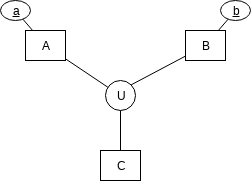
\includegraphics[scale=0.5]{e.png}
                          \end{center}

                          \begin{center}
                            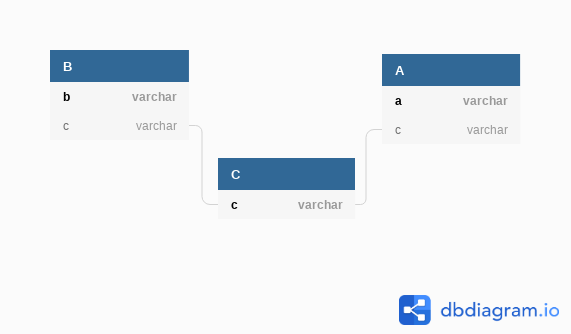
\includegraphics[scale=0.5]{e2.png}
                          \end{center}

                          \item Las superclases tienen llaves primarias idénticas.\vspace{.3cm}
                          
                          \begin{center}
                            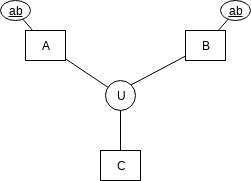
\includegraphics[scale=0.5]{d.png}
                          \end{center}

                          \begin{center}
                            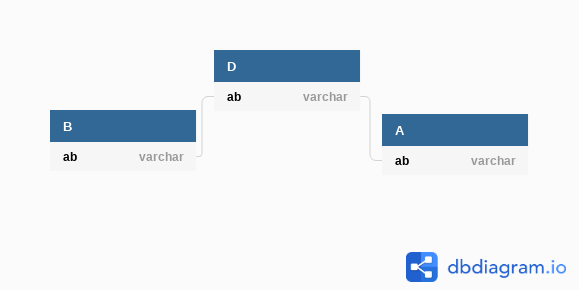
\includegraphics[scale=0.5]{d2.png}
                          \end{center}

                      \end{itemize}

                      Ejemplo:

                      \begin{itemize}
                          \item

                          \begin{center}
                            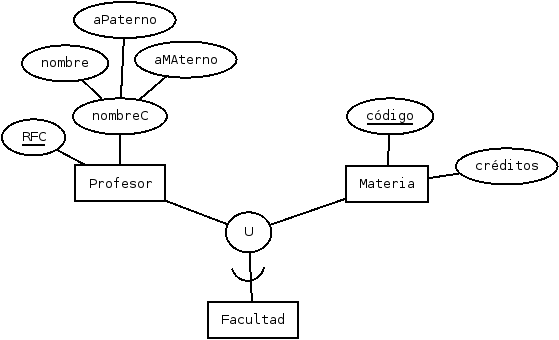
\includegraphics[scale=0.5]{cate1.png}
                          \end{center}

                          \begin{center}
                            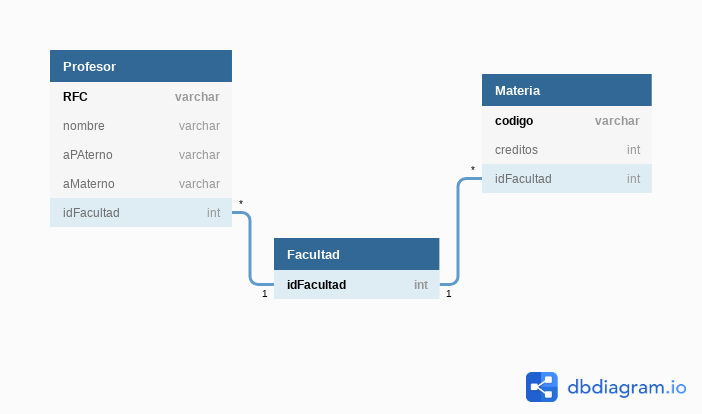
\includegraphics[scale=0.5]{categoria1.png}
                          \end{center}

                          \item 
                          
                          \begin{center}
                            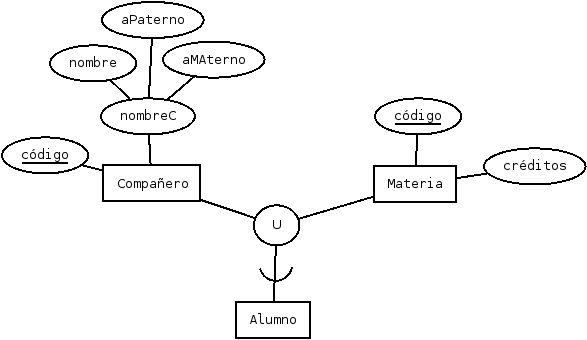
\includegraphics[scale=0.5]{cate2.png}
                          \end{center}

                          \begin{center}
                            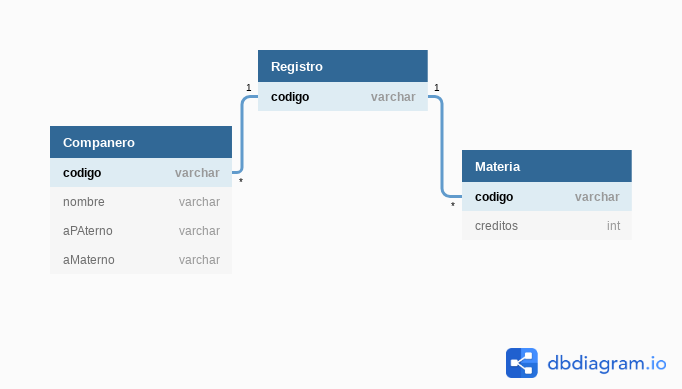
\includegraphics[scale=0.5]{categoria2.png}
                          \end{center}

                      \end{itemize}

        \end{itemize}

    \section{Modelo Relacional}

        \begin{itemize}

            \item[a.] Traduce el siguiente modelo \textbf{Entidad-Relación} a su
                      correspondiente \textbf{Modelo Relacional}:\vspace{.3cm}
                      
                      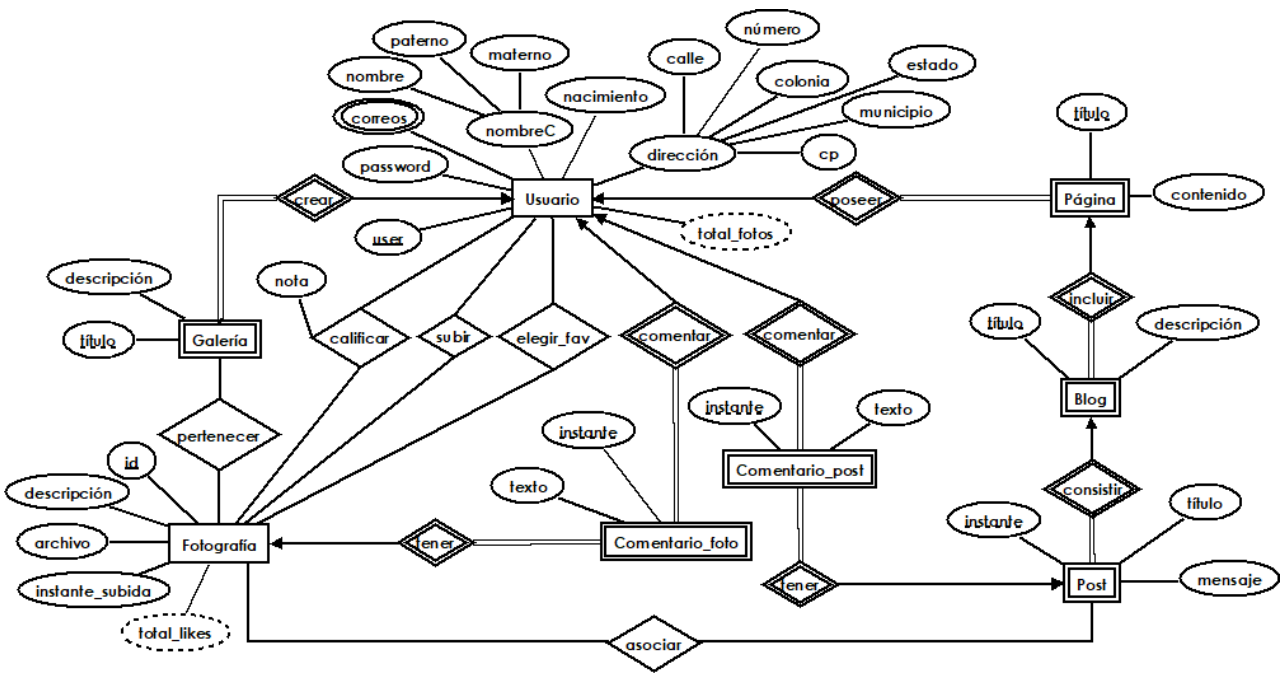
\includegraphics[scale=0.3]{ER.png}\vspace{.3cm}

                      El modelo relacional es el siguiente:\vspace{.3cm}

                      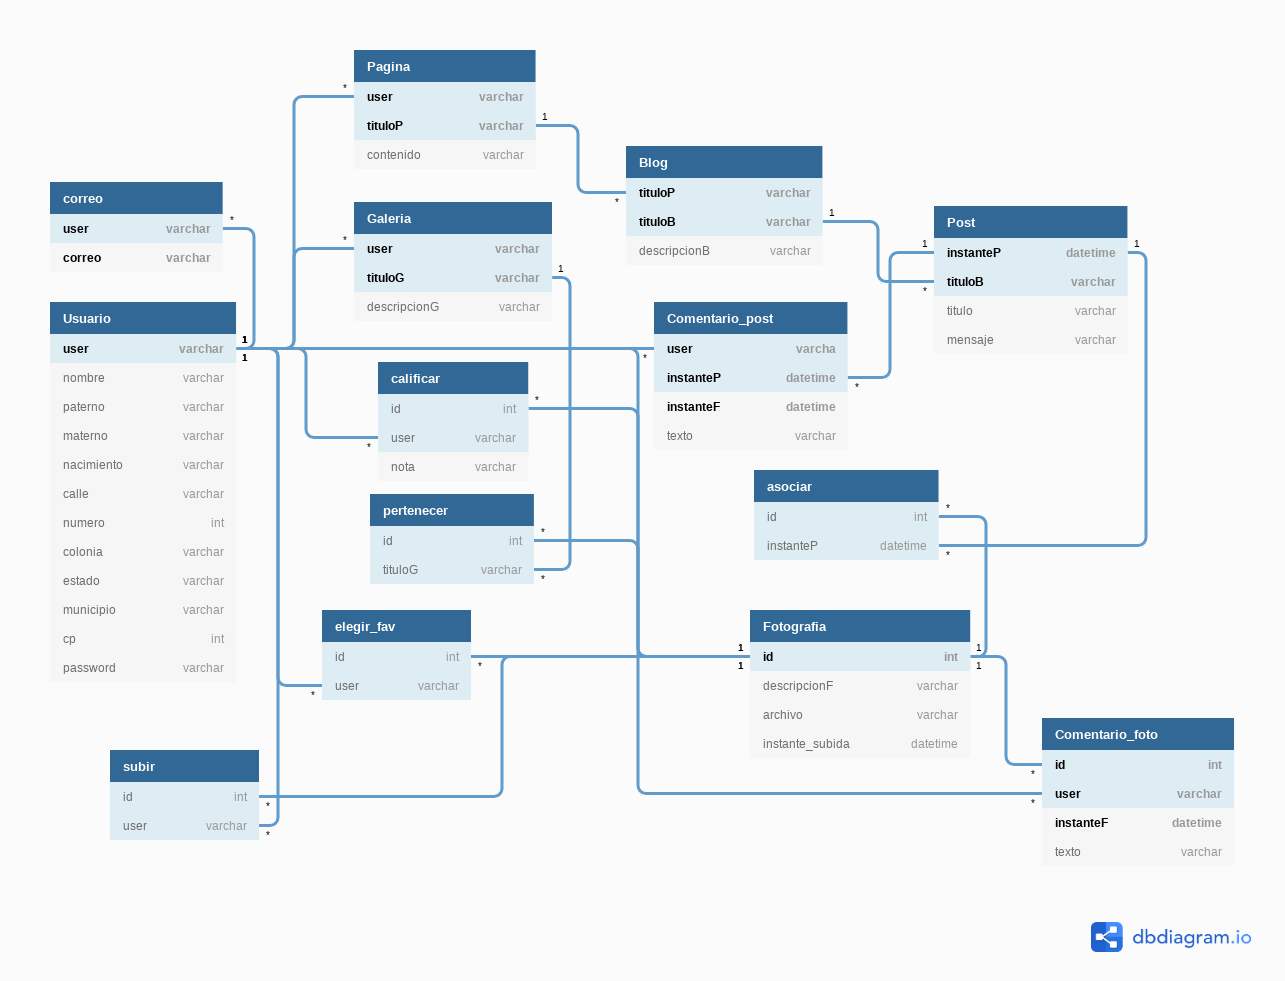
\includegraphics[scale=0.3]{Facebook.png}

Corregir en las entidades debiles se jalan todos los atributos de la entidad por ejemplo en comentario_post y blog

            \item[b.] Traduce a su correspondiente \textbf{Modelo Relacional},
                      el problema de la \textbf{Empresa de Envíos (Tarea 2)}.
                      Si realizaste alguna modificación a tu diseño original
                      (para mejorarlo), indica los cambios hechos y la
                      justificación de los mismos.

                      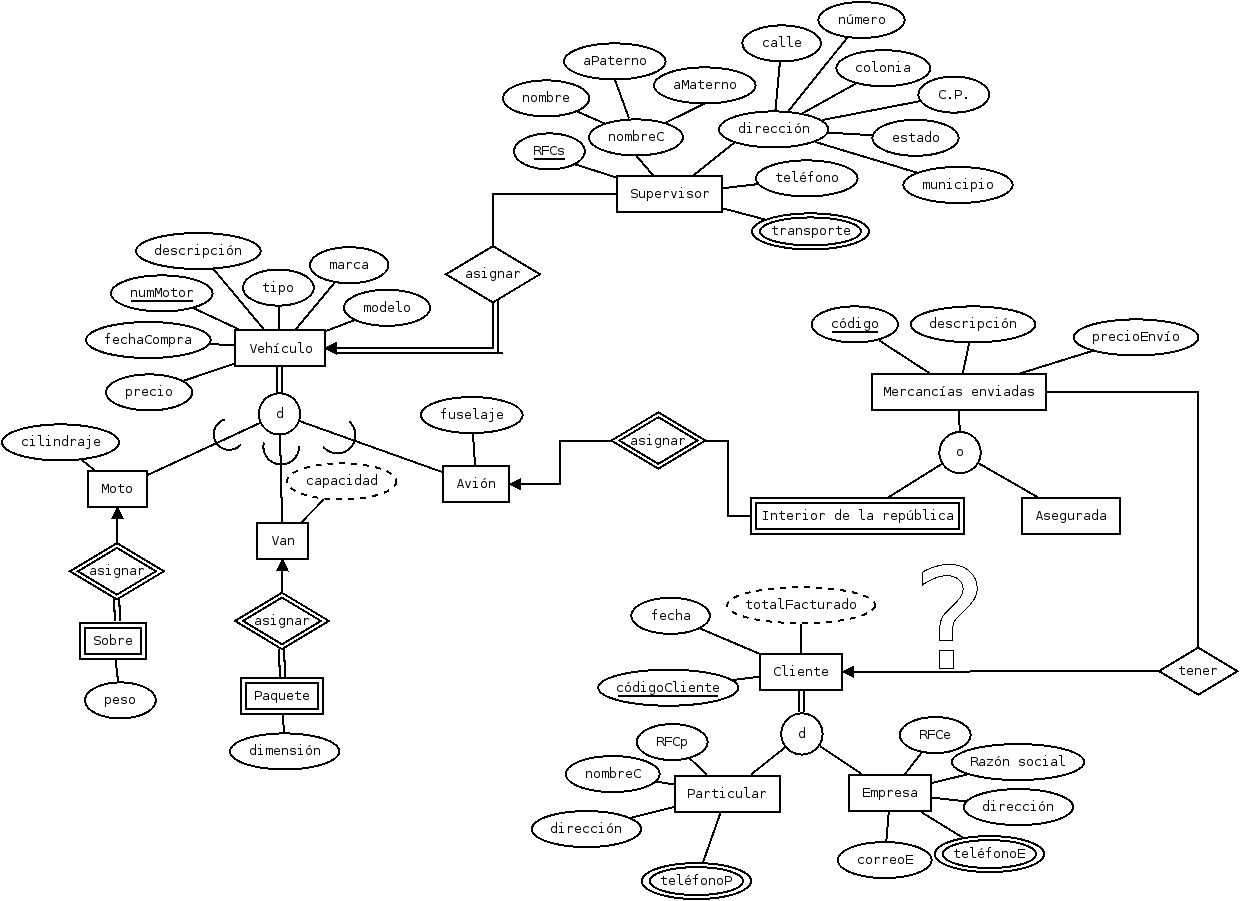
\includegraphics[scale=0.3]{empresa_envios2.png}\vspace{.3cm}

                      El modelo relacional es el siguiente:\vspace{.3cm}

                      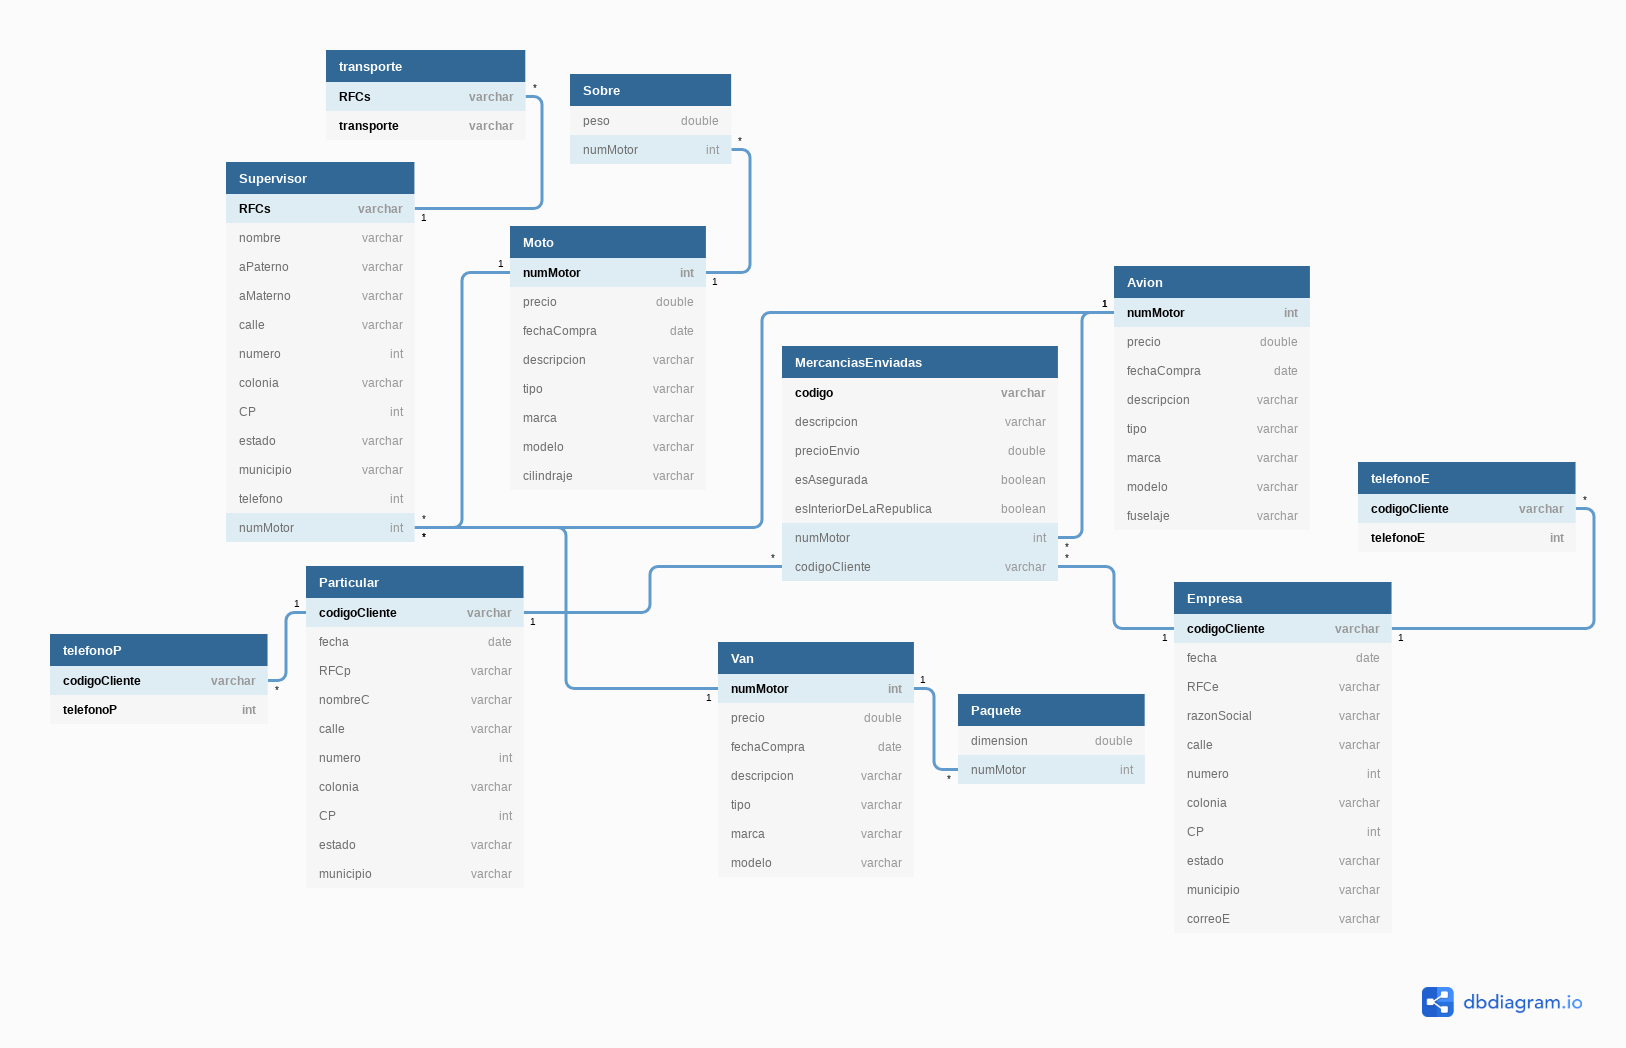
\includegraphics[scale=0.3]{Empresa_de_Envios.png}

        \end{itemize}

        Los cambios realizados que consideramos fueron en la entidad Cliente, pues 
        al tratarse de una entidad de la cual derivan dos entidades más que poseían llaves
        cada una, lo cual no está permitido, ya que se trata de una disyunción total.
        Y también renombramos otras entidades que se refierían de manera plural.


    \section{Lectura}
    Leer el artículo \textit{\textbf{Codd's 12 Rule for an RDBMS}}. Explica con
    tus propias palabras cada una de las 12 reglas de \textbf{Codd}.\vspace{.3cm}

    Indica por qué consideras que son importantes y si, haya el momento de lo
    comentado en el curso sería posible que un \textbf{SMBD} pudiera cumplir
    enteramente con lo que ahí se propone.\vspace{.3cm}

    \textbf{Reglas de Cod para un Sistema de Gestión de Bases de Datos (RDBMS)}\vspace{.3cm}

    \begin{itemize}

      \item[]\underline{REGLA 0}:  Un sistema debe calificar como relacional, base de 
                          datos y como gestor, un sistema de administración 
                          tiene que usar sus recursos o reglas para 
                          administrar la base de datos. Las 12 reglas 
                          siguientes reglas derivan de esta. \vspace{.3cm}

      \item[]\underline{REGLA 1}:  \textit{Regla de la información}: cualquier información
                          en la base de datos tiene que tener una representación 
                          única. \vspace{.3cm}

      \item[]\underline{REGLA 2}:  \textit{Regla de Garantía de acceso}: Toda información 
                          en la base de datos debe ser accesible y es necesario 
                          tener llaves primarias. \vspace{.3cm}

    \item[]\underline{REGLA 3}:  \textit{Regla de tratamiento de valores nulos}: El 
                          sistema manejador de bases de datos debe poder tratar 
                          con valores nulos, es decir que podamos tener lugares 
                          donde falte información. \vspace{.3cm}

    \item[]\underline{REGLA 4}:  \textit{Regla de catálogo}:  El sistema debe tener una 
                          opción para que los usuarios autorizados accedan a 
                          consultar la información en el mismo lenguaje que usan 
                          para acceder a la base de datos. \vspace{.3cm}

    \item[]\underline{REGLA 5}:  \textit{Regla del lenguaje}: El sistema debe aceptar 
                          al menos un lenguaje que tenga sintaxis lineal, que 
                          sea compatible con aplicaciones y que pueda realizar 
                          operaciones como manipulación, transacciones y 
                          restricciones de seguridad entre otras. \vspace{.3cm} 

    \item[]\underline{REGLA 6}:  \textit{Regla de la actualización de vista}: Todas las 
                          vistas que sufran una actualización verían ser 
                          actualizadas por el sistema. \vspace{.3cm}

    \item[]\underline{REGLA 7}:  \textit{Regla de la inserción, actualizado y borrado}: 
                          Todo sistema de bases de datos debe tener operaciones 
                          que permitan insertar, actualizar y borrar información 
                          de las tablas de datos. \vspace{.3cm}

    \item[]\underline{REGLA 8}:  \textit{Regla de la independencia física}: Cualquier 
                          cambio en el nivel físico a la base de datos no debe 
                          requerir cambios en la estructura de la base de datos.
                          \vspace{.3cm} 

    \item[]\underline{REGLA 9}:  \textit{Regla de la independencia lógica}: Cualquier 
                          cambio en el nivel lógico de la base de datos como en 
                          tablas, columnas o filas no debe requerir de cambios 
                          en la estructura de la base de datos. \vspace{.3cm}

    \item[]\underline{REGLA 10}:   \textit{Regla de la independencia de integridad}: 
                            Las restricciones de integridad deben ser declaradas 
                            aparte de las aplicaciones y se deben mostrar en el 
                            catálogo. \vspace{.3cm} 

    \item[]\underline{REGLA 11}:   \textit{Regla de la independencia de distribución}: 
                            La distribución de una parte de los datos de la base 
                            de datos debe ser invisible para los usuarios de la 
                            base de datos, es decir que no sepan que información 
                            de reparte a otras partes. \vspace{.3cm}

    \item[]\underline{REGLA 12}:   \textit{Regla de la no subversión}: El sistema debe 
                            proveer de una interfaz de bajo nivel y esa interfaz 
                            no puede tener subversiones que sobrepasen garantías 
                            de seguridad ni de integridad. \vspace{.3cm}

    \end{itemize}

  Son importantes ya que estas reglas marcan pautas para que los sistemas de datos 
  se manejen de la misma forma, es decir no tenemos sistemas donde cada quien haga 
  lo que quiera y si lo hacen se implementan son esas reglas para que todo tenga un 
  orden. \vspace{.3cm}

  Consideramos que hasta el momento del curso de han cumplido las reglas mencionadas 
  anteriormente, aunque alguna no las hayamos visto en aplicación se han mencionado 
  en algún momento del curso hasta ahora. 


  \section{Referencias}

    - $https://jisashi82.wordpress.com/2012/03/03/llave-primaria-foranea-y-candidata/$ \vspace{.3cm}

    - $https://es.wikipedia.org/wiki/Esquema_de_una_base_de_datos$ \vspace{.3cm}

    - $https://searchdatacenter.techtarget.com/es/respuesta/Definiciones-de-clave-principal-superclave-clave-foranea-y-clave-candidata-en-el-DBMS$

\end{document}
